\documentclass[12pt,a4paper]{fenbil}
\usepackage[utf8]{inputenc}
\usepackage[T1]{fontenc}
\usepackage{amsmath,amssymb,amsfonts}
\usepackage{graphicx}
\usepackage{physics}
\usepackage{siunitx}
\usepackage{tikz}
\usepackage{float}
\usepackage{xcolor}
\usepackage{fancyhdr}
\usepackage{geometry}
\usepackage{hyperref}

\geometry{margin=2.5cm}

\hypersetup{
    colorlinks=true,
    linkcolor=redM,
    filecolor=magenta,
    urlcolor=cyan,
}

\title{\textbf{Elektrik Teorisi - Hafta 4}}
\author{Ekrem Torun}
\date{14 Mart Cuma Ders Tamamı}

\begin{document}

\maketitle
\tableofcontents
\newpage

\section{Elektrik Alan ve İş}

\subsection{Elektrik Alanın İş Yapması}

Elektrik alanında bir yükün hareket ettirilmesi sırasında yapılan iş, elektrik kuvveti ve yer değiştirme ile ilişkilidir. Bir $q_0$ test yükünün elektrik alanında hareket ettirilmesi durumunda yapılan iş:

\begin{equation}
\Delta W = q_0 \Delta V
\end{equation}

Burada:
\begin{itemize}
    \item $\Delta W$: Yapılan iş
    \item $q_0$: Test yükü
    \item $\Delta V$: Potansiyel farkı
\end{itemize}

Bu ifadeyi, elektrik alan ve yer değiştirme cinsinden de yazabiliriz:

\begin{equation}
\Delta W = q_0 \Delta V = q_0 E \cos\theta \Delta L
\end{equation}

Burada:
\begin{itemize}
    \item $E$: Elektrik alan şiddeti
    \item $\theta$: Elektrik alan vektörü ile yer değiştirme vektörü arasındaki açı
    \item $\Delta L$: Yer değiştirme mesafesi
\end{itemize}

Elektrik alan ile potansiyel arasındaki ilişki:

\begin{equation}
E \cos\theta = -\frac{\Delta V}{\Delta L}
\end{equation}

Bu ifade, elektrik alanın potansiyelin negatif gradyenti olduğunu gösterir. Üç boyutlu uzayda, bu ilişki kısmi türevler kullanılarak ifade edilir:

\begin{equation}
E_x = -\frac{\partial V}{\partial x}
\end{equation}

Benzer şekilde, diğer koordinat eksenleri için:

\begin{equation}
E_y = -\frac{\partial V}{\partial y}, \quad E_z = -\frac{\partial V}{\partial z}
\end{equation}

Üç boyutlu uzayda çalıştığımız için, potansiyel birden fazla değişkene bağlıdır ve bu nedenle kısmi türevler kullanılır. Yöne bağlı olarak elektrik alan farklı değerler alabilir.

\section{Kapasitörler ve Dielektrikler}

\subsection{Kapasitans}

İki yüklü iletken arasında elektrik alan çizgileri oluşur. Bu alan çizgileri pozitif yükten negatif yüke doğru yönelir.

Kapasitans (veya kapasitör büyüklüğü), $C$ ile gösterilir ve bir kapasitörün elektrik yükü depolama yeteneğini ifade eder. Kapasitans, uygulanan potansiyel fark başına depolanan yük miktarı olarak tanımlanır:

\begin{equation}
C = \frac{Q}{V}
\end{equation}

Burada:
\begin{itemize}
    \item $C$: Kapasitans
    \item $Q$: Depolanan elektrik yükü
    \item $V$: Uygulanan potansiyel fark
\end{itemize}

Kapasitansın SI birimi Farad (F)'dır ve şu şekilde ifade edilir:

\begin{equation}
\text{Farad} = \frac{\text{Coulomb}}{\text{Volt}} = \frac{\text{C}}{\text{V}}
\end{equation}

Örneğin, 1 Farad kapasitansa sahip bir kapasitör, 1 Volt potansiyel fark uygulandığında 1 Coulomb elektrik yükü depolayabilir.

\begin{figure}[H]
    \centering
    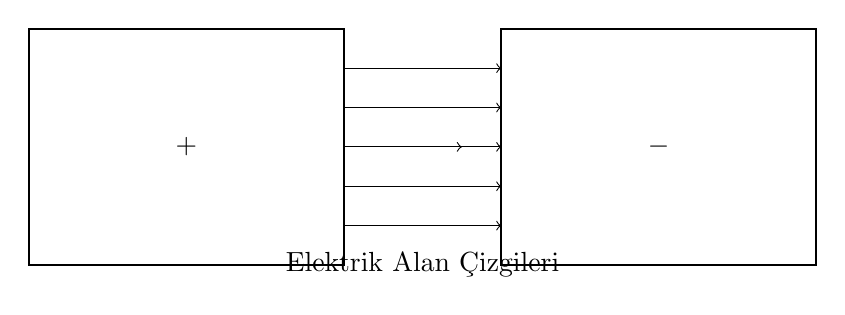
\begin{tikzpicture}
        \draw[thick] (0,0) rectangle (4,3);
        \draw[thick] (6,0) rectangle (10,3);
        \draw[->] (4.5,1.5) -- (5.5,1.5);
        \node at (2,1.5) {$+$};
        \node at (8,1.5) {$-$};
        \foreach \y in {0.5,1,1.5,2,2.5}
            \draw[->] (4,\y) -- (6,\y);
        \node at (5,0) {Elektrik Alan Çizgileri};
    \end{tikzpicture}
    \caption{Paralel Levhalı Kapasitör ve Elektrik Alan Çizgileri}
\end{figure}

İki iletken levha arasında, elektrik alan çizgileri paralel ve düzgündür (kenarlara yakın bölgeler hariç). İletkenler yüklendiğinde, fazla yükler (ekses yükler) iletkenlerin birbirlerine bakan yüzeylerinde toplanır.

\subsection{Kapasite Hesabı}

Paralel levhalı bir kapasitörün kapasitesini hesaplamak için Gauss Yasası kullanılabilir. Gauss Yasası, kapal�� bir yüzeyden geçen elektrik akısının, o yüzey içindeki toplam elektrik yüküne oranını verir:

\begin{equation}
\oint \vec{E} \cdot d\vec{S} = \frac{Q}{\varepsilon_0}
\end{equation}

Burada:
\begin{itemize}
    \item $\oint \vec{E} \cdot d\vec{S}$: Kapalı yüzeyden geçen elektrik akısı
    \item $Q$: Yüzey içindeki toplam elektrik yükü
    \item $\varepsilon_0$: Boşluğun elektrik geçirgenliği ($8.85 \times 10^{-12}$ F/m)
\end{itemize}

Düzgün elektrik alanı için, bu ifade şu şekilde sadeleşir:

\begin{equation}
\varepsilon_0 \Phi = \varepsilon_0 E A = Q
\end{equation}

Burada:
\begin{itemize}
    \item $\Phi$: Elektrik akısı
    \item $E$: Elektrik alan şiddeti
    \item $A$: Yüzey alanı
\end{itemize}

Elektrik alanı, potansiyel fark ile ilişkilidir:

\begin{equation}
V = -\int \vec{E} \cdot d\vec{l}
\end{equation}

Paralel levhalı bir kapasitör için, elektrik alanı düzgün olduğundan:

\begin{equation}
V = Ed
\end{equation}

Burada $d$, levhalar arasındaki mesafedir.

Kapasitans tanımını kullanarak:

\begin{equation}
C = \frac{Q}{V} = \frac{\varepsilon_0 E A}{Ed} = \frac{\varepsilon_0 A}{d}
\end{equation}

Bu, paralel levhalı bir kapasitörün kapasitans formülüdür.

\textbf{Önemli Not:} Kapasitansın tanımı $C = \frac{Q}{V}$ şeklindedir (tarif). Paralel levhalı kapasitör için kapasitansın tayini ise $C = \frac{\varepsilon_0 A}{d}$ formülü ile verilir.

\subsection{Elektrik Alanında Enerji Depolanması}

Bir kapasitörü yüklerken, elektrik alanında enerji depolanır. Bu enerji, kapasitörü yüklemek için yapılan işe eşittir.

Kapasitörü yüklemek için yapılan iş:

\begin{equation}
dW = V dq' = \frac{q'}{C} dq'
\end{equation}

Burada:
\begin{itemize}
    \item $dW$: Yapılan küçük iş
    \item $V$: Anlık potansiyel fark
    \item $dq'$: Küçük yük artışı
    \item $q'$: Anlık yük miktarı
\end{itemize}

Toplam iş, yük 0'dan $Q$'ya kadar değişirken yapılan işlerin toplamıdır:

\begin{equation}
W = \int_0^Q \frac{q'}{C} dq' = \frac{1}{2} \frac{Q^2}{C} = \frac{1}{2} QV = \frac{1}{2} CV^2
\end{equation}

Bu, kapasitörde depolanan enerjiyi ($U$) verir:

\begin{equation}
U = \frac{1}{2} CV^2
\end{equation}

Birim hacim başına düşen enerji miktarı (enerji yoğunluğu), $u$ ile gösterilir:

\begin{equation}
u = \frac{U}{Ad} = \frac{1}{2} \frac{CV^2}{Ad}
\end{equation}

Paralel levhalı kapasitör için $C = \frac{\varepsilon_0 A}{d}$ olduğundan:

\begin{equation}
u = \frac{1}{2} \frac{\varepsilon_0 A V^2}{d \cdot Ad} = \frac{1}{2} \varepsilon_0 \frac{V^2}{d^2}
\end{equation}

Elektrik alan $E = \frac{V}{d}$ olduğundan:

\begin{equation}
u = \frac{1}{2} \varepsilon_0 E^2
\end{equation}

Bu, elektrik alanında depolanan enerji yoğunluğunu verir. Benzer şekilde, manyetik alanda depolanan enerji yoğunluğu da manyetik alan şiddetinin karesi ile orantılıdır:

\begin{equation}
u_B = \frac{1}{2\mu_0} B^2
\end{equation}

Burada:
\begin{itemize}
    \item $u_B$: Manyetik alanda depolanan enerji yoğunluğu
    \item $\mu_0$: Boşluğun manyetik geçirgenliği
    \item $B$: Manyetik alan şiddeti
\end{itemize}

Elektromanyetik alanda toplam enerji yoğunluğu, elektrik ve manyetik enerji yoğunluklarının toplamıdır:

\begin{equation}
u_{toplam} = u_E + u_B = \frac{1}{2} \varepsilon_0 E^2 + \frac{1}{2\mu_0} B^2
\end{equation}

\end{document}